% !TeX root = RJwrapper.tex
\title{\pkg{htestClust}: A Package for Marginal Inference of Clustered Data Under Informative Cluster Size}
\author{by Mary Gregg, Somnath Datta and Douglas Lorenz}

\maketitle

\abstract{
When observations are collected in/organized into observational units, within which observations may be dependent, those observational units are often referred to as "clustered" and the data as "clustered data". Examples of clustered data include repeated measures or hierarchical shared association (e.g., individuals within families). This paper provides an overview of the R package \CRANpkg{htestClust}, a tool for the marginal analysis of such clustered data with potentially informative cluster and/or group sizes. Contained in \pkg{htestClust} are clustered data analogues to the following classical hypothesis tests: rank-sum, signed rank, $t$-, one-way ANOVA, F, Levene, Pearson/Spearman/Kendall correlation, proportion, goodness-of-fit, independence, and McNemar. Additional functions allow users to visualize and test for informative cluster size. This package has an easy-to-use interface mimicking that of classical hypothesis-testing functions in the R environment. Various features of this package are illustrated through simple examples. 
}

\section{Introduction} \label{s:intro}

Observations often occur or can be organized into units called clusters, within which those observations may be dependent. For example, individuals may be repeatedly assessed or naturally belong to some hierarchical structure like a family unit. Potential correlation among intra-cluster observations clearly invalidates the use of classical hypothesis tests for the analysis of such data. Instead, inference is generally performed using model-based methods that capture intra-cluster relationships through parametric or semi-parametric assumptions. Generalized estimating equations (GEEs) are one such approach that fit marginal generalized linear models to clustered data while making a working assumption on the correlation structure. GEE models are appealing for their flexible and robust nature, and several packages in the R environment, such as \CRANpkg{gee} \citep{carey19} and \CRANpkg{geepack} \citep{halekoh06}, offer an implementation of this method. However, GEEs and other standard methods for analysis of clustered data operate under an assumption that the number of observations within the clusters (defined as the cluster size) is ignorable. In practice, this assumption may not hold and cluster size may vary systematically in a way that carries information related to the response of interest. When this occurs data are said to have informative cluster size (ICS). Examples of ICS can be found in data related to dental health \citep{williamson03}, pregnancy studies \citep{chaurasia18}, and longitudinal rehabilitation \citep{lorenz11}, among others. For data with ICS, standard model-based methods can produce biased inference as their estimates may be overweighted in favor of larger clusters. 

A related but distinct type of informativeness occurs when the distribution of group-defining covariates varies in a way that carries information on the response. Such phenomenon has been called informative within-cluster group size (IWCGS), as well as informative covariate structure \citep{pavlou12}, sub-cluster covariate informativeness \citep{lorenz18}, and informative intra-cluster group size \citep{dutta16}. This additional informativeness may occur simultaneously with or separately from ICS, and similarly can result in the failure of standard methods to maintain appropriate nominal size \citep{huang11, dutta16}.

\citet{williamson03} developed a reweighting methodology that corrects for potential bias from cluster- or group-size informativeness. This reweighting originates from a Monte Carlo resampling process, and leads to weighting observations proportional to their inverse cluster or within-cluster group size. Correction for ICS/IWCGS was originally proposed in the context of modeling, and a number of extensions to this application have been established \citep{bible16, iosif14, mitani19, mitani20}. However, when adjustment for covariates is not of interest, this reweighting can be directly applied in the estimation of marginal parameters. Under mild conditions, such estimates are asymptotically normal, permitting Wald-type intervals and tests. This methodology has been applied to develop rank-based tests \citep{datta05, datta08, dutta16}, and tests of correlation \citep{lorenz11}, proportions \citep{gregg20}, means and variances \citep{greggdis20}. This collection of reweighted non-model-based hypothesis tests includes clustered data analogues of the following classical tests: rank-sum, signed rank, $t$-, one-way ANOVA, F, Levene, Pearson/Spearman/Kendall correlation, proportion, goodness-of-fit, independence, and McNemar.

These clustered data analogues to standard hypothesis tests provide simple and intuitive means of performing exploratory and preliminary analysis of clustered data in which the cluster and/or group size varies and is potentially informative. However, many of these tests are recent developments that are not available in a software environment. We address this deficiency through the package \pkg{htestClust}, the first R package designed as a comprehensive collection of direct, non-model-based inferential methods for analysis of clustered data with potential ICS and/or IWCGS. Introduced in this paper, \pkg{htestClust} implements the collection of methods by \citet{datta05, datta08, dutta16, lorenz11, gregg20} and \citet{greggdis20}, as well as a method by \citet{nevalainen17} that tests for the presence of informative cluster size. The syntax and output of functions contained in \pkg{htestClust} are intentionally modeled after their corresponding analogous classical function, allowing researchers to assess various marginal analyses through intuitive and user-friendly means. The rest of this paper is organized as follows. We will begin by briefly summarizing the reweighting approach developed by \citet{williamson03} and describe how its application has been used in the development of hypothesis tests of marginal parameters in clustered data. We will then provide an overview of the \pkg{htestClust} package, describe the features and structure of functions, and describe an illustrative simulated data set with informativeness. Finally, we will demonstrate \pkg{htestClust} using the example data set and close with a discussion.

\section{Methods for clustered data under informativeness} \label{s:methods}

In this section we outline the weighting methodology that corrects for bias from ICS and IWCGS, and describe the general form of the tests in \pkg{htestClust} that implement this weighting. We then summarize the balanced bootstrap design implemented in the test of ICS by \citet{nevalainen17}. 

\subsection{Notation}
Consider a sample of $M$ independent clusters, with each cluster containing $n_{i}$ potentially correlated observations, $i=1,\ldots,M$. The $j^{th}$ observation from cluster $i$ is $X_{ij}$, with $j=1,\ldots,n_{i}$. The collection of data from cluster $i$ is $\bm{V}_{i} = \{n_{i}, X_{i1}, \ldots, X_{in_{i}}\}$ and the set of all observed data is $\bm{V}=\{\bm{V}_{1}, \ldots, \bm{V}_{M} \}$. Informative cluster size is defined as inequality between the marginal distribution of the response $X$ and the distribution of $X$ conditional on cluster size: $P(X_{ij}\leq x ~|~ n_{i}=n) \neq P(X_{ij} \leq x), n=1,2,\ldots; j = 1,\ldots,n_{i}$. 

When observations within clusters belong to one of $K$ distinct groups, we define the variable $G_{ij}=k$ to represent that observation $j$ from cluster $i$ belongs to group $k$, $k=1,\ldots,K$. We let $n_{i}^{(k)}$ denote the number of observations from cluster $i$ in group $k$, and note that $n_{i}=\sum_{k=1}^{K} n_{i}^{(k)}$. We define $K_{i}^{c}=\sum_{k=1}^{K}I[n_{i}^{(k)}>0]$ to be the number of distinct groups observed in cluster $i$. When $K_i^c < K$, not all groups are observed in cluster $i$, a condition referred to as incomplete group structure. The data from cluster $i$ is now the set $\bm{V}_i=\{n_i^{(k)}, (X_{ij}, G_{ij})\}$, with observations belonging to group $k$ denoted as the set $\{ X_{i1}^{(k)},\ldots,X_{in_{i}^{(k)}}^{(k)} \}$. Informative within-cluster group size can be defined as $P\left(X_{ij}\leq x ~|~ n_{i}^{(k)}\right) \ne P\left(X_{ij}\leq x \right)$, i.e.\@ that the marginal distribution of $X$ differs from the distribution of $X$ conditional on the within-cluster group size.

\subsection{Weighting for ICS/IWCGS} \label{ss:ICS}
Let $\theta$ denote a marginal parameter to be estimated and/or tested. One approach for estimating $\theta$ is within-cluster resampling (WCR), in which one observation is randomly selected from each cluster \citep{hoffman01}. The resulting subset of data, $\bm{X}^{*}=\{X_{1}^{*}, X_{2}^{*}, \ldots, X_{M}^{*}\}$, consists of independent observations so an estimate of the parameter, $\hat{\theta}$, can be calculated using standard i.i.d.\@ methods. Clearly, this estimate is inefficient, using only a subset of the data, so the resampling process is repeated many times, creating many pseudo data sets and estimates $\hat{\theta}_q^*$. An overall estimate of $\theta$ is obtained over $Q$ resamplings ($Q$ large) by averaging the resampled estimates, $\hat{\theta}^{*}=\frac{1}{Q}\sum_{q=1}^{Q}\hat{\theta}_{q}^*$. This estimator was shown to be asymptotically normal and inference can be conducted using Wald-type intervals and tests.

The method of reweighting proposed by \citet{williamson03} derives from WCR by noting that as $M,Q \to \infty$, the overall resampled estimator converges to $\hat{\theta} = E\left[\hat{\theta}_{q}^{*} ~|~ \bm{V}\right]$ with respect to the resampling distribution. This marginalization is equivalent to averaging the resampled estimator across all realizations of the resampled data. As sampling is uniform across clusters and with equal probability within each cluster, each observation is weighted by the inverse of the associated cluster size.

The link between WCR and reweighting can be illustrated by a simple example - estimating a marginal mean. For a single resampled data set produced by WCR, the estimate of the marginal mean is the simple average, $\hat{\theta}_{q}^{*}=\frac{1}{M} \sum_{i=1}^{M} X_i^*$. Application of the marginalization calculation produces 
\begin{eqnarray*}
	\hat{\theta} & = & E \left[ \hat{\theta}_{q}^* ~|~ \bm{V}\right] \nonumber \\
	& = & \frac{1}{M} \sum_{i=1}^{M} E \left[ X_{i}^{*} | \bm{V} \right] =  \frac{1}{M} \sum_{i=1}^{M} \frac{1}{n_{i}} \sum_{j=1}^{n_{i}} X_{ij}
\end{eqnarray*}
The independence of clusters allows the expectation of the resampled estimate to be expressed as the average of the expectations. Conditioned on the observed data $\bm{V}$, the expectation of a resampled observation from a particular cluster is the average of all observations from the cluster, as the WCR process resamples observations from that cluster with equal probability. 

%\subsection{Weighting for informative within-cluster group size} \label{ss:IWCGS}
The weighting that corrects for ICS can be adapted to correct for IWCGS by modifying the underlying resampling process into a two-step procedure that marginalizes the within-cluster distribution of groups \citep{dutta16, huang11}. In this two-step resampling, we first select a group, $G_{i}^{*}$, with uniform probability from the levels of $G$ available in cluster $i$. Second, we select $X_{i}^{*}$ from the set of observations in group $k$, $\{ X_{i1}^{(k)},\ldots,X_{in_{i}^{(k)}}^{(k)} \}$, where $k$ is the group selected in the first step of the process. As in the original WCR methodology, this process is repeated for all clusters, resulting in a resampled data $\left(\bm{X}^{*}, \bm{G}^{*}\right) = \left \{ (X_{1}^{*}, G_{1}^{*}), \ldots, (X_{M}^{*}, G_{M}^{*}) \right\}$. An estimate of the parameter of interest is calculated from this resampled data. When the marginalization calculation is applied to a single WCR estimate produced by this two-step process, observations are weighted by the product of the two selection probabilities - one for the selection of a group and one for the selection of an observation within the group. Since both of these selections are made with equal probability, the weights in a given cluster are defined by the number of groups available in that cluster and the number of observations within the group:
\begin{equation*}
	w_{ij}=
	\begin{cases}
		\left(K_{i}^{c}n_{i}^{(k)}\right)^{-1}, & \text{if } n_{i}^{(k)}>0 \\
		0, 																			 & \text{otherwise.}
	\end{cases}
\end{equation*}

\subsection{Hypothesis tests of marginal parameters} \label{ss:htest}
The asymptotic normality of the estimators described in the previous section has been established under mild regularity conditions \citep{datta05, datta08, williamson03}. The tests of ranks, correlation, proportions, means and variances contained in \pkg{htestClust} all leverage this asymptotic normality through the general univariate and multivariate Wald-type forms
\begin{equation*} 
	Z = \frac{S-E\left[S\right]}{\sqrt{\hat{V}\left(S\right)}}~~~~~~~~
	\bm{X} = (\bm{S} - E(\bm{S}))^{T}\left(\hat{\bm{V}}(S)\right)^{-1}(\bm{S} - E(\bm{S})).
\end{equation*}
The statistic, $S$, differs across the various tests. However, in each of the tests $S$ is either a reweighted estimator derived through the marginalization calculation or a smooth function of such reweighted estimators. $E[S]$ is the statistic’s expected value under the null hypothesis and $\hat{V}\left(S\right)$ is an estimate of the variance of $S$. $Z$ asymptotically follows a standard normal distribution, while $\bm{X}$ asymptotically follows a chi square distribution with $K-1$ degrees of freedom.

Methods of estimating the variance of $S$ also vary across the tests. The rank-sum and signed rank tests weighted for ICS apply Hajek projections \citep{datta05, datta08}, while the tests of correlation use an approach based on the empirical variances of within-cluster averages \citep{lorenz11}. The rank-sum test weighted for IWCGS and the multi-group tests of means and variances use jackknife estimates \citep{dutta16, greggdis20}. The tests of proportions were constructed and evaluated under different variance estimation techniques including sandwich forms, method of moments, and empirical estimates. \citet{gregg20} provide a detailed examination by simulation of different variance estimation techniques in the context of estimating and testing proportions, and note that no one variance estimation technique is optimal for different types of tests. Further, the size and power of the tests in \pkg{htestClust} previously have been evaluated via simulation in the source manuscripts for each test. Predictably, each has been shown to perform well under the informativeness conditions for which they were designed to adjust.

\subsection{Testing for informative cluster size} \label{ss:ICSTest}

\citet{nevalainen17} proposed a test for ICS using a novel balanced bootstrap scheme. As it might be desirable to perform this test prior to the application of the marginal methods mentioned thus far, we have included this test for ICS in the \pkg{htestClust} package and briefly summarize it below.

Let $\bm{V}=\left(V_{1},\ldots,V_{M}\right)$ be a collection of independent clustered observations, where $V_{i}=\left(n_{i}; X_{i1},\ldots,X_{in_{i}}\right)$ is the data from cluster $i$. Assuming exchangeability of observations within clusters, the hypothesis of interest is $H_{0}: P\left(X_{ij}\leq x|n_{i}=k\right)=F(x),k=1,2,\dots;j=1,\ldots,k$, for some unknown distribution $F$. Two test statistics are proposed for testing $H_{0}$; a Kolmogorov-Smirnov type statistic takes the form
\begin{equation*}
	T_{F}=sup_{x}|\hat{F}(x)-\tilde{F}(x)|
\end{equation*}	
where $\hat{F}(x)=\frac{1}{n}\sum_{i=1}^{M}\sum_{j=1}^{n_{i}}I\left[X_{ij}\leq x\right]$ and $\tilde{F}(x)=\frac{1}{M}\sum_{i=1}^{M}\frac{1}{n_{i}}\sum_{j=1}^{n_{i}}I\left[X_{ij}\leq x\right]$. A Cramer-von Mises type alternative to $T_F$ is:
\begin{equation*}
	T_{CM}=\sum_{k\epsilon \psi} \left[kM_{k}\int{}\left(\hat{F}_{k}\left(x\right)-\hat{F}\left(x\right)\right)^{2}dx\right],
\end{equation*}
where $\psi$ represents the set of unique cluster sizes, $M_{k}$ represents the number of clusters of size $k$, and $\hat{F}_{k}(x)=\frac{1}{kM_{k}}\sum_{i=1}^{M}\sum_{j=1}^{n_{i}}I\left[n_{i}=k, X_{ij}\leq x\right]$. $T_{CM}$ is suggested for use when there is a small number of distinct cluster sizes, as it tends to be more powerful. $T_{F}$ is preferred when the number of distinct cluster sizes is large and the number of clusters with those sizes is small, as $T_{CM}$ tends to be too liberal.

The bootstrap scheme, which is employed for either statistic, is as follows. For iteration $b,b=1,\ldots,B$,  \
\begin{enumerate}
	\item	Permute observations within each cluster.
	\item Resample clusters from the permuted data by performing the following for $i = 1,\ldots, M$: 
	\begin{enumerate}
		\item Randomly select a cluster $i^{*},i^{*}=1,\ldots,M$. 
		\item If $n_{i^{*}} \geq n_{i}$, form the $i^{th}$ bootstrapped cluster from the first $n_{i}$ observation from cluster $i^{*}$; e.g., $V_{bi}^{*}=\left(n_{i}; X_{i^{*}1},\ldots,X_{i^{*}n_{i}}\right)$.
		\item 	If $n_{i}^{*}<n_{i}$, form the $i^{th}$ bootstrapped cluster by merging observations from the resampled cluster $i^{*}$ and observations from the closest ‘matching’ cluster to cluster $i^{*}$; e.g., $V_{bi}^{*}=\left(n_{i}; X_{i^{*}1},\ldots,X_{i^{*} n_{i}^{*}},X_{k(n_{i}^{*}+1)},\ldots,X_{kn_{i}}\right)$, where $k=\arg\min_{k} \{D(V_{i^{*}}, V_{k}): n_{k} \geq n_{i}\}$. The closest matching cluster is determined by minimum distance calculated by $D\left(V_{i},V_{j}\right)=\left(\min\{n_{i}, n_{j}\}\right)^{-1} \sum_{k=1}^{\min\{n_{i}, n_{j}\}}\left(X_{ik}-X_{jk}\right)^{2}$.
	\end{enumerate}
	\item Calculate the test statistic from the collection of bootstrapped clusters, $T_{b}^{*}=T\left(\bm{V}_{b}^{*}\right)$, $\bm{V}_{b}^{*}=\left(V_{b1}^{*},\ldots,V_{bM}^{*}\right)$.  	
\end{enumerate}

The approximate p-value is then obtained from the sample of bootstrapped test statistics by $\frac{1}{B}\sum_{b=1}^{B}I\left[T_{b}^{*} \geq T\right]$, where $T$ is the desired test statistic calculated from the original data.

\section[Overview of htestClust]{Overview of \pkg{htestClust}} \label{s:overview}

\pkg{htestClust} includes ten functions for conducting different hypothesis tests under ICS, one function for visualizing informativeness in cluster size, and a simulated hypothetical data set to illustrate the use of the functions. We first note that, at the time of this publication, we are aware of only two other R packages available on CRAN that provide functions for analyzing data under ICS and IWCGS: \CRANpkg{clusrank} \citep{jiang18} and \CRANpkg{ClusterRankTest} \citep{dutta16b}. Each of these packages provides functionality only for rank-based tests for clustered data, i.e. clustered data analogues of the well-known Wilcoxon signed rank and rank sum tests. We know of no other R package that includes the broad range of tests of means, proportions, variances, and correlations in addition to these rank-based tests that is provided by \pkg{htestClust}.

\subsection[Functions and Behavior]{Package functions, syntax, and output} \label{ss:func}

With the exception of the test of informative cluster size, each of the hypothesis testing functions implemented in \pkg{htestClust} has a well-known analogue test for i.i.d.\@ data (Table \ref{t:pckFun}). As such, the syntax and output of the functions in \pkg{htestClust} are designed to conform with that of the analogous i.i.d.\@ functions from the R \pkg{stats} library. A notable but necessary departure from this correspondence is that the \pkg{htestClust} functions require as input (1) a variable identifying the clusters as an argument in the data set or (2) a cluster-level summary of the data.

\begin{table}[t!]
	\footnotesize
	\centering
	\renewcommand{\arraystretch}{1.25}
	\begin{tabular}{lll}
		\textbf{htestClust} function		 & Reweighted test(s)														& Classical analogue function \\
		\hline 
		\texttt{chisqtestClust()}	   & Chi squared goodness of fit, independence	  & \texttt{chisq.test()} \\
		\texttt{cortestClust()}	 	   & Correlation        													& \texttt{cor.test()}   \\
		\texttt{icstestClust()}			 & Test of ICS																	& NA	\\
		\texttt{levenetestClust()}	 & $K$-group test of variance       						& \texttt{leveneTest()} \\
		\texttt{mcnemartestClust()}	 & Homogeneity																	& \texttt{mcnemar.test()} \\
		\texttt{onewaytestClust()}	 & $K$-group mean equality		     						  & \texttt{oneway.test()} \\
		\texttt{proptestClust()}		 & Proportion 									  							& \texttt{prop.test()} \\
		\texttt{ttestClust()}				 & Test of means (one/two group, paired)				& \texttt{t.test()}  \\
		\texttt{vartestClust()}			 & 2-group test of variance       							& \texttt{var.test()} \\	
		\texttt{wilcoxtestClust()}   & Rank sum, signed rank 												& \texttt{wilcox.test()} \\
		\hline																		
	\end{tabular}
	\caption{\label{t:pckFun} Hypothesis testing functions available in the \textbf{htestClust} package. Each row gives the name of a \textbf{htestClust} function, the reweighted test the function performs, and the R function that executes the corresponding classical analogue test. All classical analogue functions are available in R through the \pkg{stats} package, except for \texttt{leveneTest()}, which is included in the \CRANpkg{car} package.}
\end{table}

As an example, consider the syntax for the \pkg{stats} and \pkg{htestClust} functions for conducting a test of a single proportion:
\begin{example}	
	prop.test(x, n, p = NULL, alternative = c("two.sided", "less", "greater"),
	conf.level = 0.95, correct = TRUE)
	
	proptestClust(x, id, p = NULL, alternative = c("two.sided", "less",
	"greater"), variance = c("sand.null", "sand.est", "emp", "MoM"),
	conf.level = 0.95)
\end{example}
The \pkg{stats} library function \code{prop.test} does not operate on variables in a data frame, but instead takes summary counts as its input. Argument \code{x} can be a scalar representing the number of binomial successes, whence \code{n} is required as the number of binomial trials. Alternatively, \code{x} can be a one-dimensional table or matrix with two entries, whence \code{n} is omitted. The remaining arguments customize the test in ways familiar to most users.

The function \code{proptestClust} from \pkg{htestClust} operates on binary variables in a data frame or on cluster-level summary counts. In this function, \code{x} may be a binary variable measured over clusters, wherein \code{id} is required as a vector of cluster identifiers. Alternatively, \code{x} may instead be a two-dimensional table of within-cluster counts of failures and successes, wherein \code{id} is omitted. As previously noted, several options are available for variance estimation; these may be selected by the user through the \code{variance} argument. Additional customization of the test is as in \code{prop.test}.

Each of the testing functions in \pkg{htestClust} has been constructed in this vein -- parallel to the analogous \pkg{stats} function with contingencies necessary for clustered data. \pkg{htestClust} functions accept vector input that designates the response, grouping (if necessary), and clustering variables. However, for convenience, many functions are designed with a secondary interface accepting tables or formulas. Like their \pkg{stats} package analogues, \pkg{htestClust} testing functions produce \code{list} objects of class \code{htest} for which the \code{print} method behaves in the usual way.

\code{icsPlot} provides a simple method for illustrating informative cluster size, providing a visual supplement to the results of the test of ICS, \code{icstestClust}. Briefly, \code{icsPlot} plots a within-cluster summary statistic of a variable, such as a mean, against the size of each cluster. For quantitative variables, \code{icsPlot} produces a scatterplot of a within-cluster measure of location (mean, median) or variation (SD, variance, IQR, range) against cluster size. For a categorical variable, a barplot of within-cluster proportions is produced.
\subsection[Data Set]{Simulated example data set} \label{ss:dataset}

\pkg{htestClust} includes a simulated data set named \code{screen8} of clustered observations with informativeness, created under a hypothetical scenario we briefly describe here. A large school district has conducted a voluntary comprehensive exit survey for students graduating elementary school, collecting demographic, biometric, and academic performance data. The clustering mechanism for these data are the schools, with students comprising the observations within clusters.

The school district has offered an incentive program to boost participation, wherein schools having higher participation rates are rewarded with priority status for classroom and technology upgrades for the new academic year. This incentive introduces the potential for ICS -- resource-poor schools may exhibit greater participation (larger cluster sizes) but also tend to have students with poorer health metrics and standardized test scores. 

\code{screen8} contains data from 2224 students from 73 schools in this district. Cluster sizes -- the number of students participating in the exit survey at each school -- ranged from 17 to 50, with a median of 30. The first few lines of the data are printed below, followed by the tabulated number of participants from each school and a summary of the cluster sizes. Table \ref{t:screen8} provides details on the variables in the data set. 

\begin{example}	
	R> library(htestClust)
	R> data(screen8)
	R> head(screen8)	
	sch.id stud.id age gender height weight math read phq2 qfit qfit.s activity
	1      1       1  15      M     65    136   69   75    3   Q2     Q2    other
	2      1       2  14      M     66    135   80   57    2   Q4     Q3    other
	3      1       3  15      M     65    146   60   85    0   Q2     Q3   sports
	4      1       4  15      M     68    156   70   83    1   Q3     Q2    other
	5      1       5  15      M     68    170   66   60    1   Q2     Q2   sports
	6      1       6  14      M     63    109   84   62    0   Q1     Q1 academic
	
	R> (tab <- table(screen8$sch.id)) 
	1  2  3  4  5  6  7  8  9 10 11 12 13 14 15 16 17 18 19 20 21 22 23 24 25 26 
	35 32 26 33 23 25 27 21 39 28 32 38 35 24 29 27 36 29 38 39 25 30 36 29 46 27
	...
	
	R> summary(as.vector(tab))
	Min. 1st Qu.  Median    Mean 3rd Qu.    Max. 
	17.00   25.00   30.00   30.47   36.00   50.00
\end{example}
\begin{table}[t!]
	\footnotesize
	\centering
	\renewcommand{\arraystretch}{1.25}
	\begin{tabular}{p{0.1\linewidth} p{0.85\linewidth}}
		\textbf{Variable} 		 & \textbf{Description}	\\
		\hline 
		\texttt{sch.id}	   & School identification variable	 \\
		\texttt{stud.id}	   & Student identification variable within school	 \\
		\texttt{age}	   & Student age in years	 \\
		\texttt{gender}	   & Student gender \\
		\texttt{height}	   & Student height in inches \\
		\texttt{weight}	   & Student weight in lbs \\
		\texttt{math}	   & Student score on standardized math test \\
		\texttt{read}	   & Student score on standardized reading test \\
		\texttt{phq2}	   & Ordinal (0-6) score from a mental health screening. Higher scores correspond to higher levels of depression \\
		\texttt{qfit}	   & Age-adjusted fitness quartile from physical health assessment taken at end of school year \\
		\texttt{qfit.s}	   & Age-adjusted fitness quartile from physical health assessment taken at beginning of school year \\
		\texttt{activity}  & Student after-school activity \\
		\hline																		
	\end{tabular}
	\caption{\label{t:screen8} Variables in \code{screen8} data set. Each row gives the name of a variable included in the \code{screen8} data set and its associated description.}
\end{table}
\pagebreak

\section{Examples} \label{s:examples}

In this section, we demonstrate usage of the functions in \pkg{htestClust} using the \code{screen8} data set. Our illustration is not comprehensive, but users can learn more about functions not covered here by browsing the associated help files. To motivate the demonstration, we'll investigate the following questions:
\begin{enumerate}
	\item Is the proportion of students having ``proficient'' standardized math test scores (65 or greater) more than 0.75?
	\item Are participation in extracurricular activity and gender independent?
	\item Are mean standardized math test scores different between male and female students?
	\item Are mean standardized reading test scores different among groups defined by extracurricular activities?
\end{enumerate}

\subsection[Evaluating ICS]{Evaluating informative cluster size} \label{ss:icseval}

Before addressing these questions, we illustrate how to assess the potential informativeness of cluster size in the data set, starting by visualizing ICS through the \code{icsPlot} function. The arguments to \code{icsPlot} specify the variable of interest, a cluster-identifying variable, and a summary function to be applied to the variable within each cluster. This summary can be any of \samp{obs}, \samp{mean}, \samp{median}, \samp{var}, \samp{IQR}, \samp{range}, \samp{prop}, producing plots of the observations themselves, measure of location, or measures of variation against cluster size. Option \samp{prop} can only be used when the variable of interest is a factor, so numerically coded categorical variables must be converted to factors. Standard R graphical parameters can also be specified when calling \code{icsPlot()}.
\begin{example}	
	R> ### Figure 1
	R> par(mfrow = c(1,2))
	R> icsPlot(x = screen8$math, id = screen8$sch.id, FUN = "mean", pch = 20)
	R> icsPlot(x = screen8$read, id = screen8$sch.id, FUN = "mean", pch = 20)
	
	R> ### Figure 2
	R> layout(mat = matrix(c(1, 2), nrow = 1, ncol = 2),
	+        heights = c(1, 2), # Heights of the two rows
	+        widths = c(2, 2.5))
	R> par(mar = c(5, 4, 1, 0))
	R> icsPlot(x = screen8$gender, id = screen8$sch.id, FUN = "prop", 
	+        ylab = "P(Female)", pch = 20)
	R> par(mar = c(5, 4, 1, 5))
	R> icsPlot(x = screen8$activity, id = screen8$sch.id, FUN = "prop", 
	+         legend = TRUE,
	+         args.legend = list(x = "topright", bty = "n", inset=c(-0.32, 0)))
\end{example}
Figures \ref{f:ScorebyClSize} and \ref{f:GrpbyClSize} show potential informativeness in cluster size for the \code{screen8} data. Cluster size appears to be negatively associated with average standardized test scores but positively associated with the proportion of male students and the proportion participating in sports-related extracurricular activities.
\label{s:screen8}
\begin{figure*}[t!]
	\setlength{\fboxsep}{0pt}%
	\setlength{\fboxrule}{0pt}%
	\begin{center}
		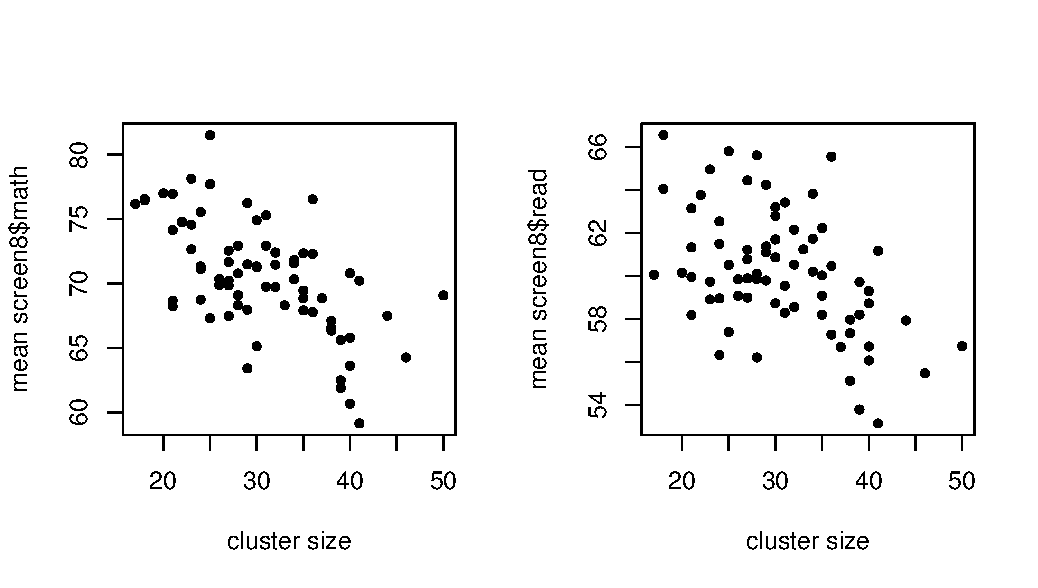
\includegraphics[scale=.6] {MathRead.pdf}
		\caption{Average scores in maths and reading by cluster size in \code{screen8} data.}
		\label{f:ScorebyClSize}
	\end{center}
\end{figure*}
\begin{figure*}[t!]
	\setlength{\fboxsep}{0pt}%
	\setlength{\fboxrule}{0pt}%
	\begin{center}
		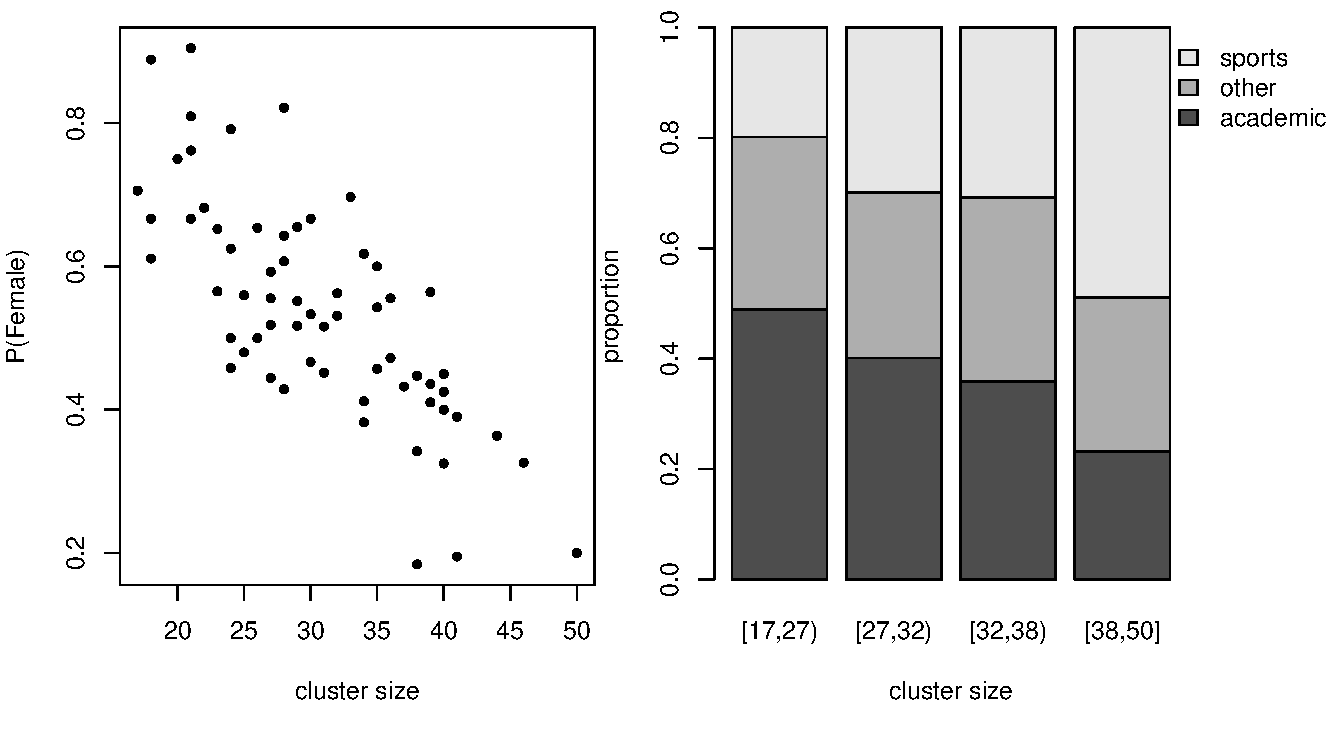
\includegraphics[scale=0.5] {GrpbyClSize.pdf}
		\caption{Plots of categorical variables by cluster size in \code{screen8} data. Proportion of female students decreases with cluster size (left), whereas student participation in sports-related extracurricular activities increases with cluster size (right).}
		\label{f:GrpbyClSize}
	\end{center}
\end{figure*}
These empirical results can be verified using the test for ICS, implemented through the function \code{icstestClust}, as illustrated below. The result of this test suggests that cluster size is informative for standardized math test scores. Cluster size is also informative for standardized reading test scores, gender, and sports as an extracurricular activity ($p < .001$, results not shown). 
\begin{example}		
	R> set.seed(100)
	R> ics.math <- icstestClust(screen8$math, screen8$sch.id, B = 1000, 
	+    print.it = FALSE)
	
	R> ics.math
	Test of informative cluster size (TF)
	data:  screen8$math
	TF = 0.029686, p-value < 2.2e-16
\end{example}
Within the \code{icstestClust} function, the type of test statistic, TF or TCM as detailed earlier, is specified using the \code{test.method} argument, and the number of bootstrap loops by argument \code{B}.  Argument \code{print.it} is a logical indicating whether to print the progress of the bootstrap procedure. We note that the need for bootstrap resampling in \code{icstestClust} can make its implementation computationally expensive.

\subsection[Marginal proportion test]{Testing a marginal proportion} \label{ss:proptest}

The first question of interest suggests a one-sample test of a proportion via \code{proptestClust}. We specify a one-sided alternative and use the default sandwich variance estimator evaluated at the null value of the proportion (\code{variance = "sand.null"}), shown to perform best for this test \citep{gregg20}.
\begin{example}	
	R> screen8$math.p <- 1*(screen8$math >= 65)
	R> proptestClust(screen8$math.p, screen8$sch.id, p = .75, alternative = "great")
	Cluster-weighted proportion test with variance est: sand.null
	
	data:  screen8$math.p, M = 73
	z = 0.70159, p-value = 0.2415
	alternative hypothesis: true p is greater than 0.75
	95 percent confidence interval:
	0.7311459 1.0000000
	sample estimates:
	Cluster-weighted proportion 
	0.7640235 
\end{example}
As noted earlier, \pkg{htestClust} functions produce objects of class \code{htest}, producing familiar output through the \code{print} method for such objects. We conclude that the proportion of students with proficient math test scores is not greater than 0.75.

In the case that all clusters have a size of 1, the results of \pkg{htestClust} functions will be in general correspondence with that of the classical analogue test, though exact results will differ slightly due to the reweighted tests relying on asymptotics. This is demonstrated through the following example. 
\begin{example}
	R> set.seed(123)
	R> x <- rbinom(100, size = 1, p = 0.7)
	R> id <- 1:100
	R> proptestClust(x, id)
	
	Cluster-weighted proportion test with variance est: sand.null
	
	data:  x, M = 100
	z = 4.2, p-value = 2.669e-05
	alternative hypothesis: true p is not equal to 0.5
	95 percent confidence interval:
	0.6120018 0.8079982
	sample estimates:
	Cluster-weighted proportion 
	0.71 
	
	R> prop.test(sum(x), length(x))
	
	1-sample proportions test with continuity correction
	
	data:  sum(x) out of length(x), null probability 0.5
	X-squared = 16.81, df = 1, p-value = 4.132e-05
	alternative hypothesis: true p is not equal to 0.5
	95 percent confidence interval:
	0.6093752 0.7942336
	sample estimates:
	p 
	0.71 
\end{example}

\subsection[Independence test]{Test of independence}

The second question suggests a test of independence of extracurricular activity and gender. We start by producing cluster-weighted estimates of the proportion of students participating in each activity within each gender.
\begin{example}	
	R> tab <- table(screen8$gender, screen8$activity, screen8$sch.id) 
	R> ptab <- prop.table(tab, c(1,3))
	R> apply(ptab, c(1,2), mean)
	academic     other    sports
	F  0.3952102 0.2968473 0.3079425
	M  0.3790267 0.3186699 0.3023035
\end{example}
The cluster-weighted proportions appear roughly similar, and we can test using \code{chisqtestClust}. Here, the default method of variance estimation is method of moments (\code{variance = "MoM"}), demonstrated to be best for the test of independence \citep{gregg20}.
\begin{example}	
	R> chisqtestClust(screen8$gender, screen8$activity, screen8$sch.id)
	Cluster-weighted Chi-squared test of independence with variance est:
	MoM
	
	data:  screen8$gender and screen8$activity, M = 73
	X-squared = 1.6131, df = 2, p-value = 0.4464
\end{example}

Before proceeding to the next analysis, we note that further evidence of ICS in the \code{screen8} data can be demonstrated by implementing the standard chi-squared test for this question, which suggests that females were more likely to participate in academic extracurricular activities and males in sports.

\begin{example}	
	R> prop.table(table(screen8$gender, screen8$activity), 1)
	academic     other    sports
	F  0.3891323 0.2979842 0.3128834
	M  0.3370268 0.3120960 0.3508772
	
	R> chisq.test(screen8$gender, screen8$activity)
	Pearson's Chi-squared test
	
	data:  screen8$gender and screen8$activity
	X-squared = 6.9303, df = 2, p-value = 0.03127
\end{example}

\subsection[Quantitative tests]{Tests of quantitative variables for two or more groups} \label{ss:quant}

We compare math test scores between males and females using the \code{ttestClust} function. We conclude that mean standardized test scores are equivalent between males and females, a departure from the conclusion reached by the standard t test (p < .001, results not shown). 
\begin{example}	
	R> ttestClust(math ~ gender, id = sch.id, data = screen8)
	
	Two sample group-weighted test of means
	
	data:  math by gender, M = 73
	z = 1.3495, p-value = 0.1772
	alternative hypothesis: true difference in means is not equal to 0
	95 percent confidence interval:
	-0.2234259  1.2111344
	sample estimates:
	weighted mean in group F weighted mean in group M 
	70.75124                 70.25739
\end{example}
Even though this test does not make use of the $t$ distribution, we have named it as such to parallel the standard $t$-test means (\code{t.test} in R). Multi-group tests of quantitative parameters in \pkg{htestClust} implement jackknife variance estimation, so specification of variance estimation method is not necessary. In addition to the formula implementation used above, we note that \code{ttestClust} can also accept vectors of data and cluster identifiers for each of the two groups. 

An alternative approach to this comparison, particularly if test scores were skewed in any way, would be a rank-based test. \code{wilcoxtestClust} implements the group-weighted analogue of the Wilcoxon test, which we use as an alternative method for the comparison of math test scores between males and females.
\begin{example}	
	R> wilcoxtestClust(math ~ gender, id = sch.id, data = screen8, method = "group")
	Group-weighted rank sum test
	
	data:  math by gender, M = 73
	z = -1.3799, p-value = 0.1676
	alternative hypothesis: true location shift is not equal to 0
\end{example}
Our conclusion is the same as with the reweighted test of means. We note that this test requires estimation of the cluster-weighted empirical cumulative distribution \citep{dutta16} as well as jackknife variance estimation, so there is an added measure of computational expense in using \code{wilcoxtestClust}.

Finally, we compare reading test scores among the three groups defined by extracurricular activity, using \code{onewaytestClust}. Mean standardized reading test scores are not appreciably different among extracurricular activity groups.
\begin{example}	
	R> onewaytestClust(read ~ activity, id = sch.id, data = screen8)
	Reweighted one-way analysis of means for clustered data
	
	data:  read and activity, M = 73
	X-squared = 1.3191, df = 2, p-value = 0.5171
	sample estimates:
	academic    other   sports 
	60.11498 60.40785 59.69659
\end{example}
We have not shown the full functionality of the above-demonstrated functions, nor the \pkg{htestClust} functions for testing correlation, marginal homogeneity, and variance listed in Table \ref{t:pckFun}. Their syntax and usage is similar and fully documented with examples in the help files.


%% -- Summary/conclusions/discussion -------------------------------------------

\section{Discussion} \label{sec:summary}
Standard model-based inference of clustered data can be biased when cluster or group size is informative. Reweighting methods that correct for this bias have been established and a number of authors have applied such weighting to develop direct hypothesis tests of marginal parameters in clustered data. Such tests can be interpreted as clustered analogues to common classical statistical tests, and include methods related to ranks, correlation, proportions, means and variances. While these methods are effective and intuitive, all but a few of these tests have remained inaccessible to many researchers due to an absence of convenient software.

In this paper we introduced \pkg{htestClust}, which is the first R package designed as a comprehensive library of inferential methods appropriate for clustered data with ICS/IWCGS. Most functions in \pkg{htestClust} perform hypothesis tests for clustered data that have an analogous classical form, and the interface of the package has been designed to reflect this relationship. Function syntax has been purposefully structured to resemble that of functions available in the native R environment that perform the analogous classical tests. Many functions have been designed with a secondary interface that operates through table or formula input, allowing flexibility in data structure. In addition to the hypothesis tests of marginal parameters, \pkg{htestClust} also includes functions to visualize potential informativeness and test for ICS. These tools allow analysts to explore the effect and degree of informativeness in their data. 

With the exception of the test for ICS, the hypothesis tests performed by \pkg{htestClust} are derived through the asymptotic normality of reweighted parameters, and their asymptotic convergence is indexed by the number of clusters. As such, their use should only be considered when the number of clusters is sufficiently large (at least 30). Additionally, these methods retain a cluster-based marginal interpretation, making them appropriate when clusters, rather than intra-cluster observations, are the unit of interest. The marginal nature of these tests provides researchers with an analysis corresponding to a snapshot in time. If analysis of temporal aspects or effects of additional covariates is desired, readers might instead consider reweighted model-based methods such as those by \citet{bible16}, \citet{neuhaus11}, and \citet{wang11}. Future research will also be devoted to developing tests adjusting for informativeness due to quantitative covariates measured at the individual-within-cluster level.

\pkg{htestClust} is a tool to facilitate the analysis of clustered data, and we have designed its use to be accessible and intuitive. While the inferential methods performed by this package have been developed to correct for the biasing effects of ICS/IWCGS, they remain applicable when fluctuations of cluster or group size are unrelated to the outcome of interest. As such, this package is an effective resource for researchers addressing marginal analyses in clustered data with any variation in the cluster and/or group sizes. 


\section*{Computational details}

%\begin{leftbar}
%If necessary or useful, information about certain computational details
%such as version numbers, operating systems, or compilers could be included
%in an unnumbered section. Also, auxiliary packages (say, for visualizations,
%maps, tables, \dots) that are not cited in the main text can be credited here.
%\end{leftbar}

The results in this paper were obtained using
R~4.0.3 with the
\pkg{MASS}~7.3.51 package. 



\section*{Acknowledgments}

The authors would like to thank Lucas Koepke and an anonymous reviewer for their thorough review and insightful comments that improved the quality of this manuscript.


\bibliography{gregg}

\address{Mary Gregg\\
	Department of Bioinformatics and Biostatistics\\
	University of Louisville\\
	485 East Gray Street\\
	Louisville, KY 40202, USA\\
	ORCiD: 0000-0003-2991-6939\\
	\email{mary.gregg@louisville.edu}}

\address{Somnath Datta\\
	Department of Biostatistics\\
	University of Florida\\
	2004 Mowry Rd \\
	P.O. Box 117450\\
	Gainesville, FL 32611 USA\\
	ORCiD: 0000-0003-4381-1842\\
	\email{somnath.datta@ufl.edu}}

\address{Douglas Lorenz\\
	Department of Bioinformatics and Biostatistics\\
	University of Louisville\\
	485 East Gray Street\\
	Louisville, KY 40202, USA\\
	ORCiD: 0000-0001-8114-0926\\
	\email{djlore01@louisville.edu}}